%%%%%%%%%%%%%%%%%%%%%%%%%%%%%%%%%%%%%%%%%
% Beamer Presentation
% Juraj Fulir
% Faculty of Electrical Engineering and Computing
% University of Zagreb
%
% Project Presentation
%
%
%%%%%%%%%%%%%%%%%%%%%%%%%%%%%%%%%%%%%%%%%

%----------------------------------------------------------------------------------------
%	PACKAGES AND THEMES
%----------------------------------------------------------------------------------------

\documentclass{beamer}

\mode<presentation> {

% The Beamer class comes with a number of default slide themes
% which change the colors and layouts of slides. Below this is a list
% of all the themes, uncomment each in turn to see what they look like.

%\usetheme{default}
%\usetheme{AnnArbor}
%\usetheme{Antibes}
%\usetheme{Bergen}
%\usetheme{Berkeley}
%\usetheme{Berlin}
%\usetheme{Boadilla}
%\usetheme{CambridgeUS}
%\usetheme{Copenhagen}
%\usetheme{Darmstadt}
%\usetheme{Dresden}
%\usetheme{Frankfurt}
%\usetheme{Goettingen}
%\usetheme{Hannover}
%\usetheme{Ilmenau}
%\usetheme{JuanLesPins}
%\usetheme{Luebeck}
\usetheme{Madrid}
%\usetheme{Malmoe}
%\usetheme{Marburg}
%\usetheme{Montpellier}
%\usetheme{PaloAlto}
%\usetheme{Pittsburgh}
%\usetheme{Rochester}
%\usetheme{Singapore}
%\usetheme{Szeged}
%\usetheme{Warsaw}

% As well as themes, the Beamer class has a number of color themes
% for any slide theme. Uncomment each of these in turn to see how it
% changes the colors of your current slide theme.

%\usecolortheme{albatross}
%\usecolortheme{beaver}
%\usecolortheme{beetle}
%\usecolortheme{crane}
%\usecolortheme{dolphin}
%\usecolortheme{dove}
%\usecolortheme{fly}
%\usecolortheme{lily}
%\usecolortheme{orchid}
%\usecolortheme{rose}
%\usecolortheme{seagull}
%\usecolortheme{seahorse}
%\usecolortheme{whale}
%\usecolortheme{wolverine}

%\setbeamertemplate{footline} % To remove the footer line in all slides uncomment this line
%\setbeamertemplate{footline}[page number] % To replace the footer line in all slides with a simple slide count uncomment this line

%\setbeamertemplate{navigation symbols}{} % To remove the navigation symbols from the bottom of all slides uncomment this line
}

\usepackage{graphicx} % Allows including images
\usepackage{booktabs} % Allows the use of \toprule, \midrule and \bottomrule in tables
\usepackage[utf8]{inputenc}
\usepackage[croatian]{babel}
\usepackage{listings}
\usepackage{textpos}
\usepackage{amsthm}
\usepackage{multirow}
\usepackage{hyperref}
\usepackage{subcaption}
\usepackage{wrapfig}

\graphicspath{ {./res/} }

%----------------------------------------------------------------------------------------
%	TITLE PAGE
%----------------------------------------------------------------------------------------

\title[Diplomski rad]{Optimizirane aktivacijske funkcije klasifikatora temeljenog na umjetnim neuronskim mrežama u domeni implementacijskih napada na kriptografske uređaje}

\author{Juraj Fulir}
\institute[UNIZG, FER, ZEMRIS]
{
\includegraphics[height=2cm,width=2cm]{unizg.pdf}\\
Sveučilište u Zagrebu \\
Fakultet elektrotehnike i računarstva \\ 
Zavod za elektroniku, mikroelektroniku, računalne i inteligentne sustave \\
\medskip
\textit{Mentor: prof.\ dr.\ sc.\ Domagoj Jakobović,\\ Karlo Knežević, mag.\ ing.\ comp.\ } \\
\medskip
\textit{DIPLOMSKI RAD}
}
\date{4. srpnja 2019.}

\begin{document}

\begin{frame}
\titlepage
\end{frame}

\begin{frame}
\frametitle{Sadržaj}
\tableofcontents
\end{frame}

%----------------------------------------------------------------------------------------
%	PRESENTATION SLIDES
%----------------------------------------------------------------------------------------

%------------------------------------------------
\section{Uvod} 
%------------------------------------------------

\begin{frame}
\frametitle{Uvod}
\begin{itemize}
\item Kriptografski uređaji su nezamjenjiv element digitalne infrastrukture modernog društva
\item Pametne kartice (bankovne kartice, identifikacijski dokumenti)
\item Kriptoalgoritam štiti povjerljive podatke
\item Dobar kriptoalgoritam može biti siguran, no sklopovlje emitira informacije u okolinu

\end{itemize}

\end{frame}

%------------------------------------------------
\section{Implementacijski napadi} 
%------------------------------------------------

\begin{frame}
\frametitle{Implementacijski napadi}
\begin{itemize}
\item Pretpostavka: emitirane informacije i sadržaj registara su korelirani
\item Cilj: otkriti tajni ključ na temelju izmjerenih emisija (razlučitelj)
\item Uvjeti: uređaj mora biti uključen i mora sadržavati tajni ključ
\item Postoji više vrsta napada, grupirani su u aktivne i pasivne
\end{itemize}

\end{frame}

%------------------------------------------------
\subsection{Napad analizom potrošnje električne energije} 
%------------------------------------------------

\begin{frame}
\frametitle{Analiza potrošnje električne energije}
\begin{itemize}
\item Ideja: iskoristiti korelaciju između potrošnje el. energije uređaja i podataka zapisanih na uređaju
\item Napad koji je iznimno teško detektirati
\item Postoji više pristupa, među najpoznatijim je diferencijalna analiza potrošnje el. energije
\end{itemize}

\end{frame}

%------------------------------------------------
\subsection{Podatkovni skupovi} 
%------------------------------------------------

\begin{frame}
\frametitle{Podatkovni skupovi}
\begin{itemize}
\item Napad na AES-128
\item Ulaz: trag potrošnje el. energije, reduciran Pearsonovom korelacijom
\item Izlaz: predikcija vrijednosti okteta ili Hammingove težine
\item DPAv2: FPGA implementacija
\item DPAv4: programska implementacija
\end{itemize}
\begin{figure}
\centering
\begin{subfigure}{.49\textwidth}
  \centering
  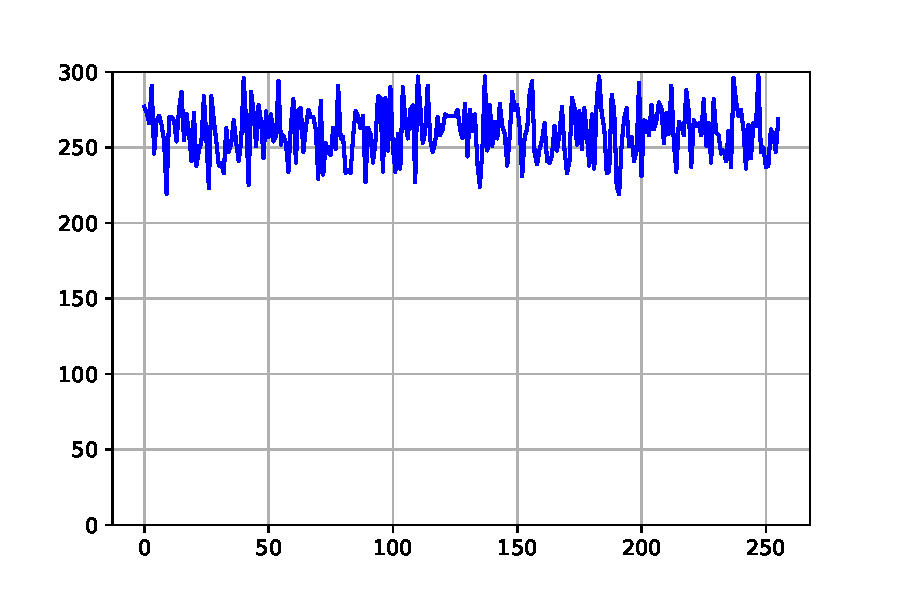
\includegraphics[width=\linewidth]{ds_nl256_tr_outputs.pdf}
  \caption{Vrijednosti okteta, DPAv4}
\end{subfigure}
\begin{subfigure}{.49\textwidth}
  \centering
  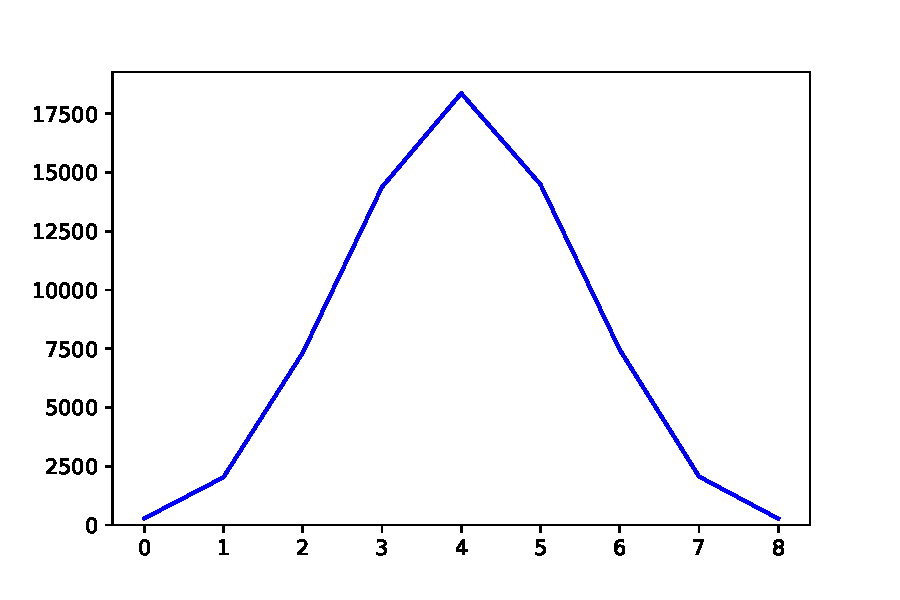
\includegraphics[width=\linewidth]{ds_nl9_tr_outputs.pdf}
  \caption{Hammongove težine, DPAv4}
\end{subfigure}
\end{figure}

\end{frame}

%------------------------------------------------
\section{Odabir arhitekture} 
%------------------------------------------------

\begin{frame}
\frametitle{Odabir arhitekture}

Neuronska mreža

\begin{itemize}
\item Arhitektura: potpuno povezana, relativno plitka (do 4 skrivena sloja)
\item Optimizacija: Adam, smanjivanje stope učenja, rano zaustavljanje
\item Regularizacija: L2, normalizacija grupom
\end{itemize}

Pretraga hiperparametara po rešetki

\begin{itemize}
\item Optimizacija stope učenja i L2 koeficijenta
\item Usporedba arhitektura i aktivacijskih funkcija
\item Odabir arhitektura, optimalnih za većinu funkcija
\item F1 mjera -- harmonijska sredina preciznosti i odziva (makro)
\end{itemize}
\end{frame}

%------------------------------------------------
\subsection{Rezultati DPAv4 (oktet)}
%------------------------------------------------

\begin{frame}
\frametitle{Rezultati DPAv4 (oktet)}

\begin{figure}
\centering
\begin{subfigure}{.48\textwidth}
  \centering
  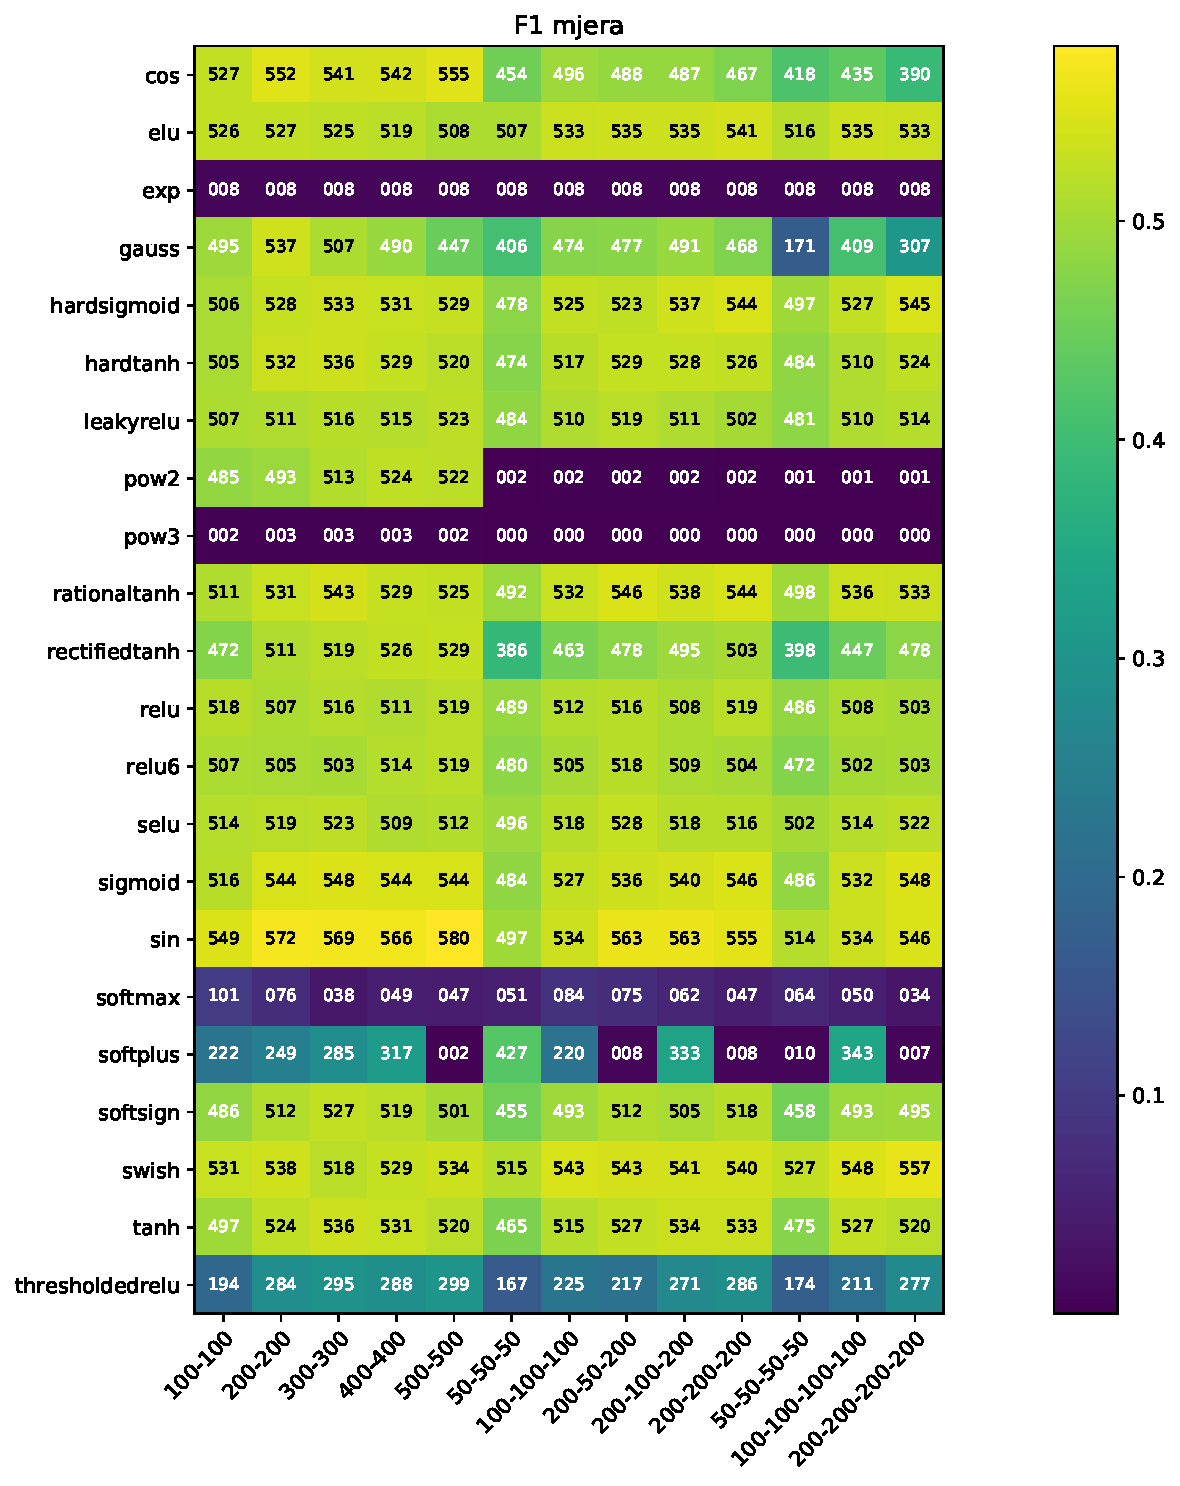
\includegraphics[width=\linewidth]{greedy_256_f1.pdf}
\end{subfigure}
\begin{subfigure}{.5\textwidth}
  \centering
  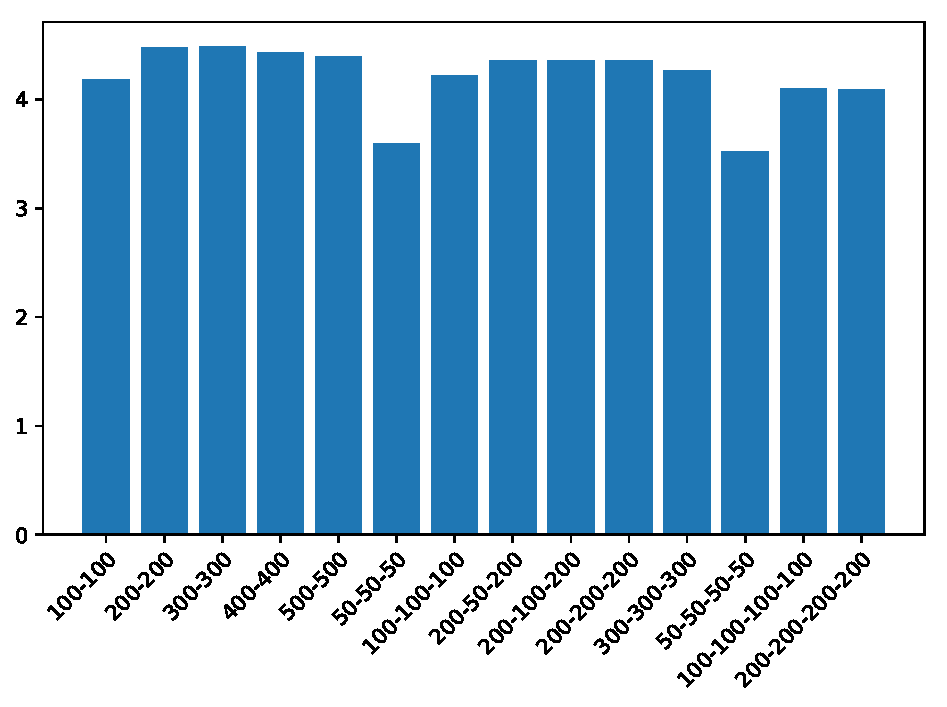
\includegraphics[width=\linewidth]{greedy_256_arch_quality.pdf}
\end{subfigure}
\end{figure}

\end{frame}

%------------------------------------------------
\subsection{Rezultati DPAv4 (HW)}
%------------------------------------------------

\begin{frame}
\frametitle{Rezultati DPAv4 (HW)}

\begin{figure}
\centering
\begin{subfigure}{.48\textwidth}
  \centering
  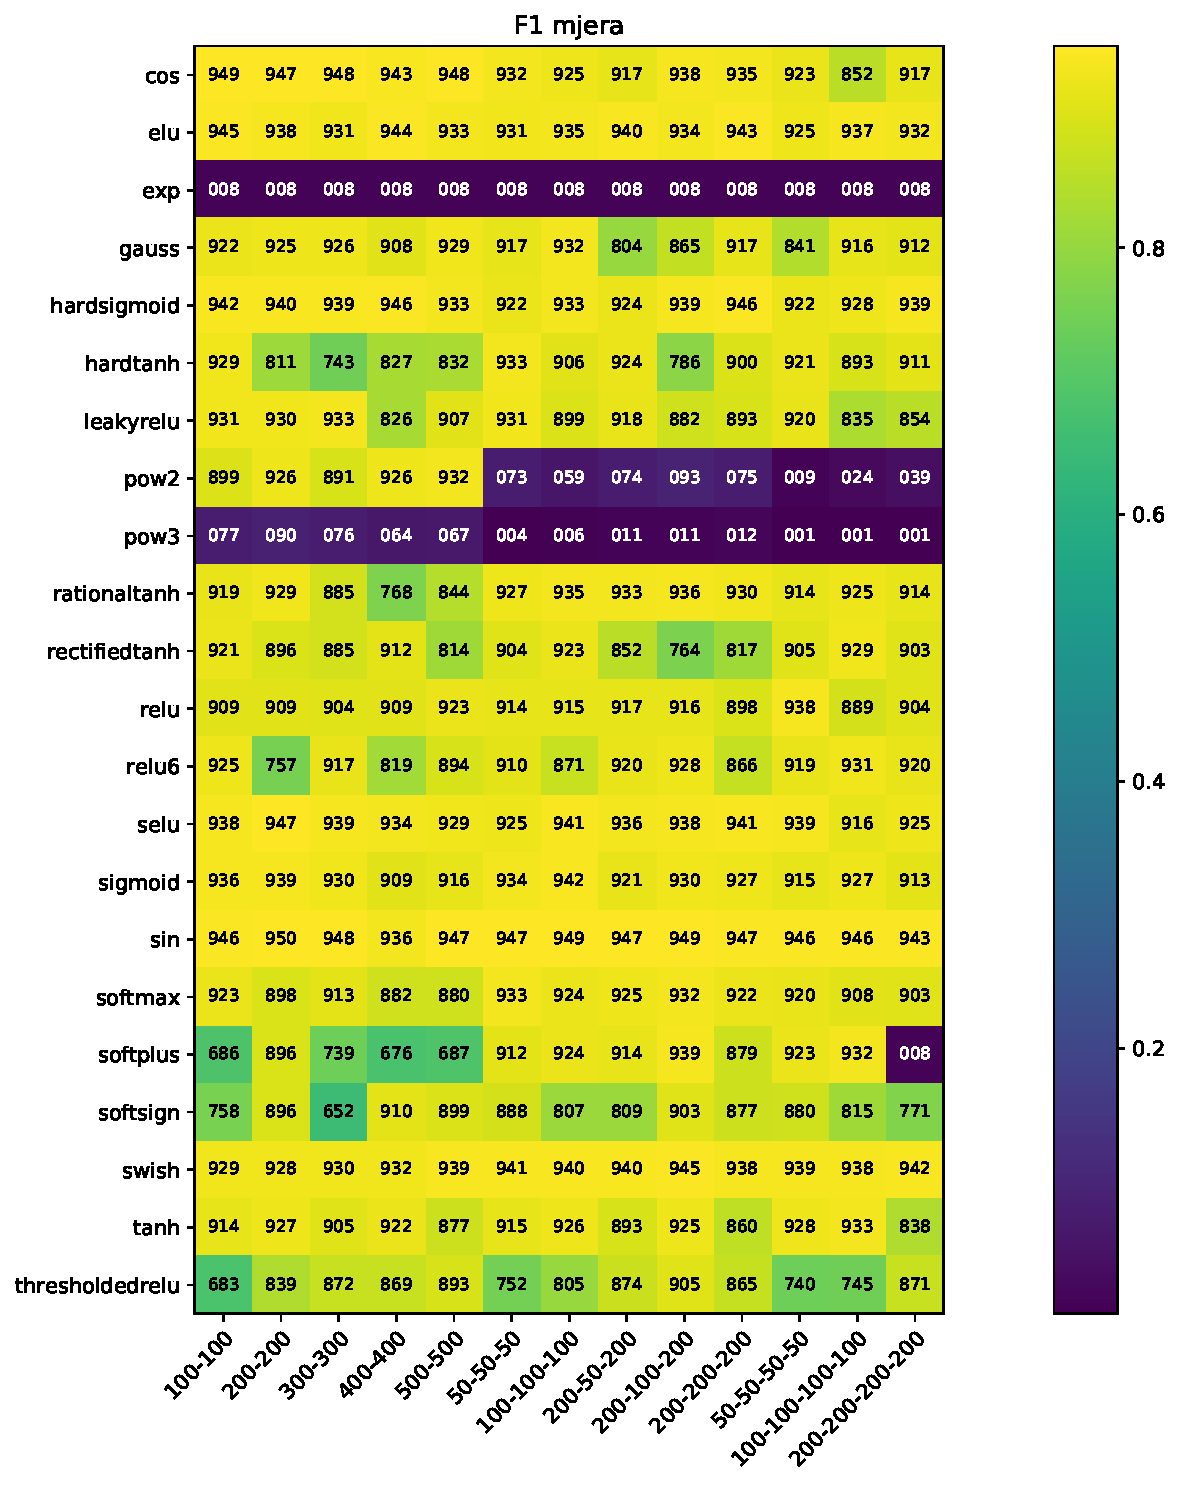
\includegraphics[width=\linewidth]{greedy_9_f1.pdf}
\end{subfigure}
\begin{subfigure}{.5\textwidth}
  \centering
  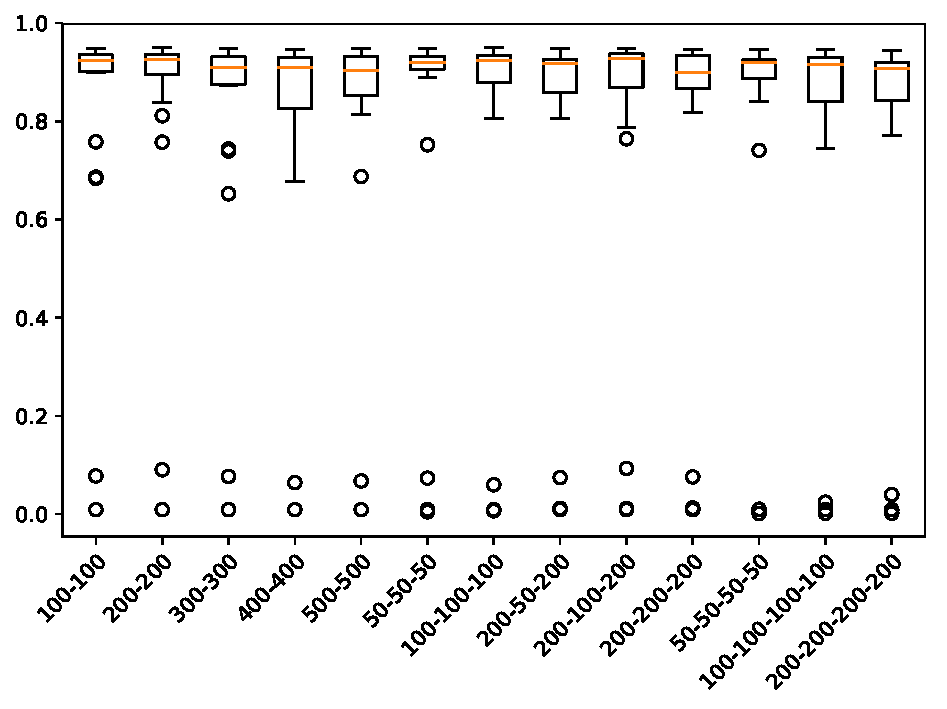
\includegraphics[width=\linewidth]{greedy_9_arch_quality.pdf}
\end{subfigure}
\end{figure}

\end{frame}

%------------------------------------------------
\section{Izgradnja aktivacijskih funkcija}
%------------------------------------------------

\begin{frame}
\frametitle{Izgradnja aktivacijskih funkcija}

\begin{wrapfigure}{r}{3cm}
  \includegraphics[width=\linewidth]{LReLU_tree.pdf}
  \caption{Funkcija LReLU}
\end{wrapfigure}

Genetsko programiranje

\begin{itemize}
\item Populacijski algoritam
\item Tabu lista
\item Paralelna evaluacija
\end{itemize}

Evolucija aktivacijske funkcije

\begin{itemize}
\item AF kao simboličko stablo
\item Čvorovi: ulaz, konstanta, matematičke op. i popularne AF
\item Po nekoliko operatora križanja i mutacije
\item Usporedba rezultata po veličini tabu liste s prethodno ostvarenim (rešetkom)
\end{itemize}

\end{frame}

%------------------------------------------------
\subsection{Rezultati DPAv4 (oktet)}
%------------------------------------------------

\begin{frame}
\frametitle{Rezultati DPAv4 (oktet)}

\begin{figure}
\centering
\begin{subfigure}{.49\textwidth}
  \centering
  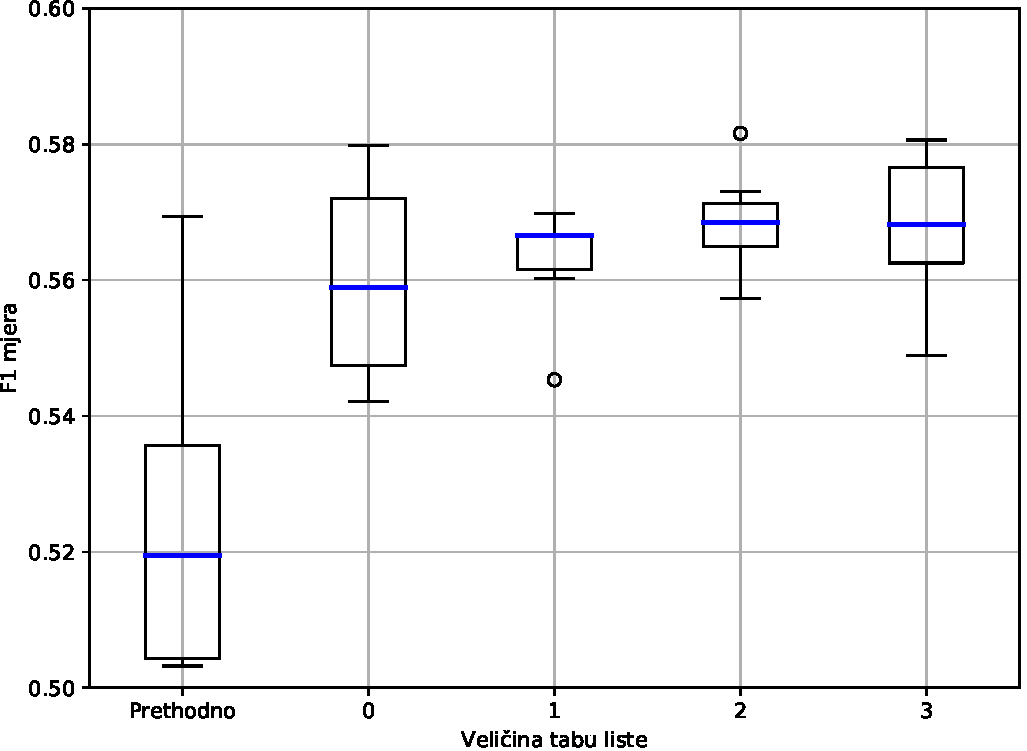
\includegraphics[width=\linewidth]{GP_256class_f1_plus.pdf}
\end{subfigure}
\begin{subfigure}{.49\textwidth}
  \centering
  \begin{subfigure}{\linewidth}
    \centering
    \tiny $(\cos(x-4.153574932708071))^2$
    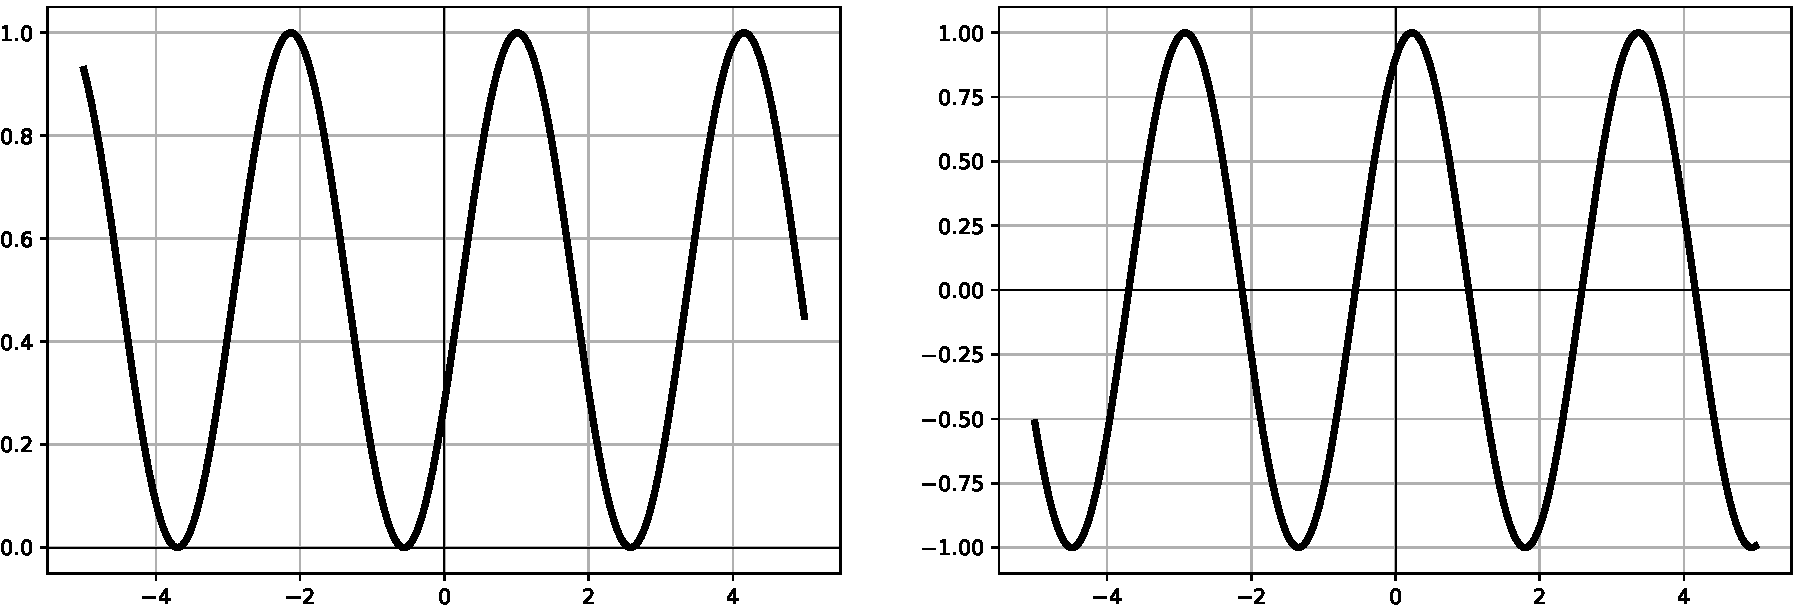
\includegraphics[width=\linewidth]{dpav2_gp_f1.pdf}
  \end{subfigure}
  \begin{subfigure}{\linewidth}
    \centering
    \vspace{2mm}
    \tiny $elu (elu (\min (1.0,\min (1.0,hsigm (x)) \cdot 0.8102254104210314) \cdot \sin (x)))$
    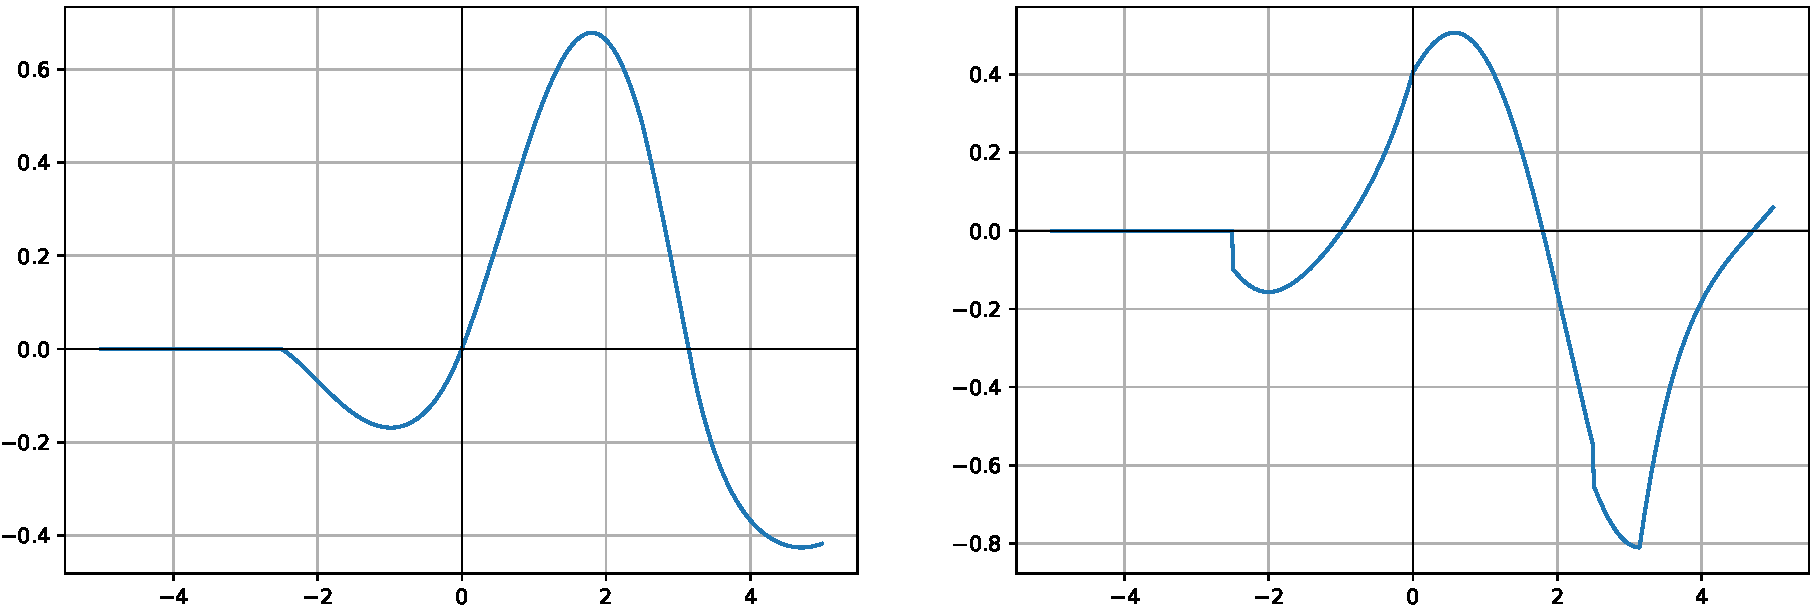
\includegraphics[width=\linewidth]{dpav2_gp_f2.pdf}
  \end{subfigure}
  \begin{subfigure}{\linewidth}
    \centering
    \vspace{2mm}
    \tiny $(\cos(1.0 + x))^2$
    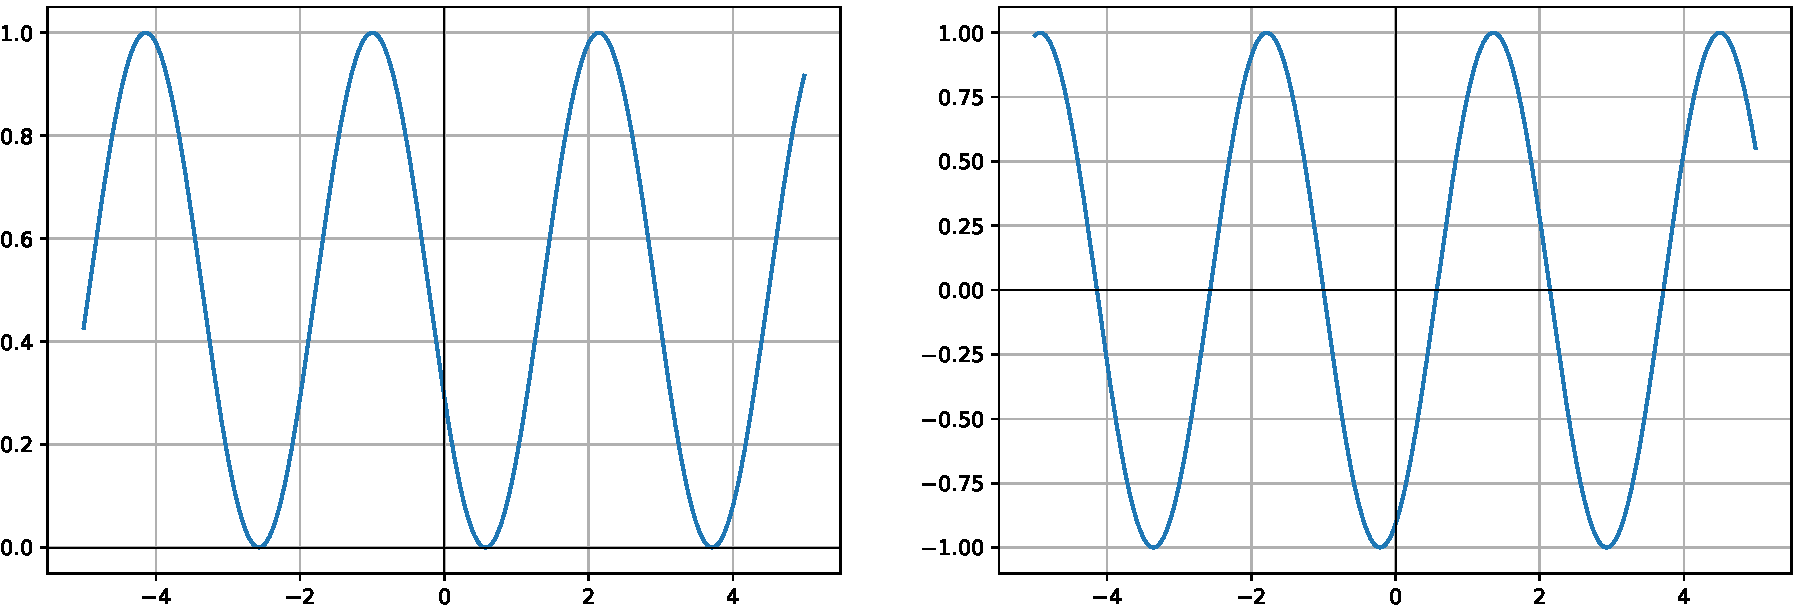
\includegraphics[width=\linewidth]{dpav2_gp_f3.pdf}
  \end{subfigure}
\end{subfigure}
\end{figure}

\end{frame}

%------------------------------------------------
\subsection{Rezultati DPAv4 (HW)}
%------------------------------------------------

\begin{frame}
\frametitle{Rezultati DPAv4 (HW)}

\begin{figure}
\centering
\begin{subfigure}{.49\textwidth}
  \centering
  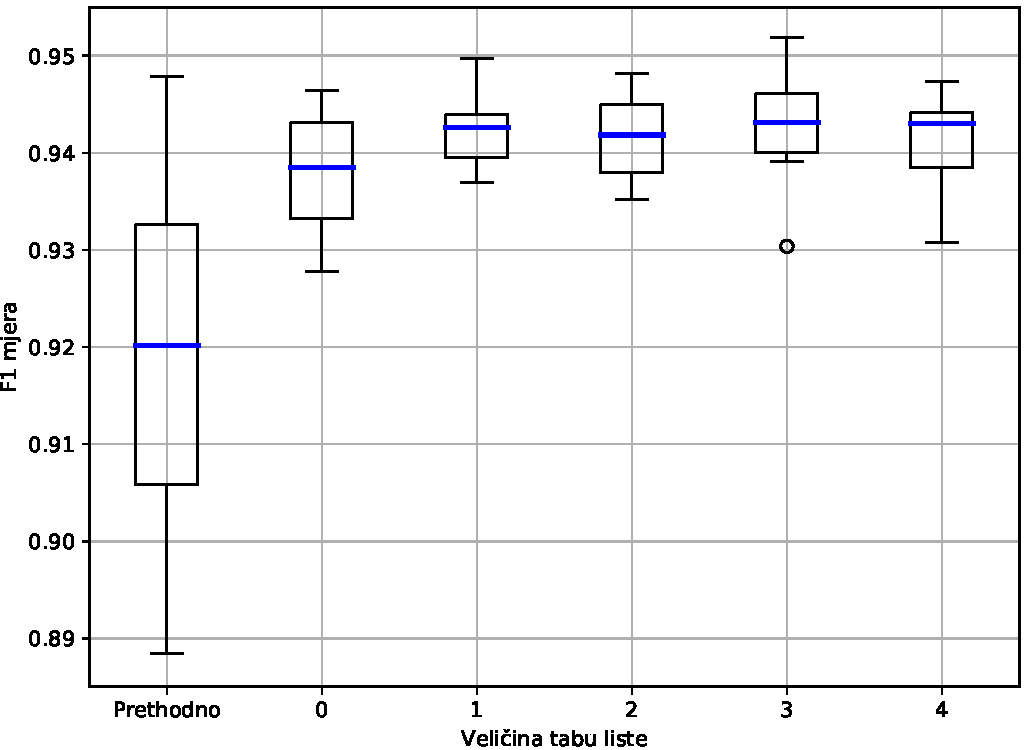
\includegraphics[width=\linewidth]{GP_9class_f1_plus.pdf}
\end{subfigure}
\begin{subfigure}{.49\textwidth}
  \centering
  \begin{subfigure}{\linewidth}
    \centering
    \tiny $\sin (\min (\sin (\min (x,0.5068783911631836) + 1.0),-0.9990098031722499) + x)$
    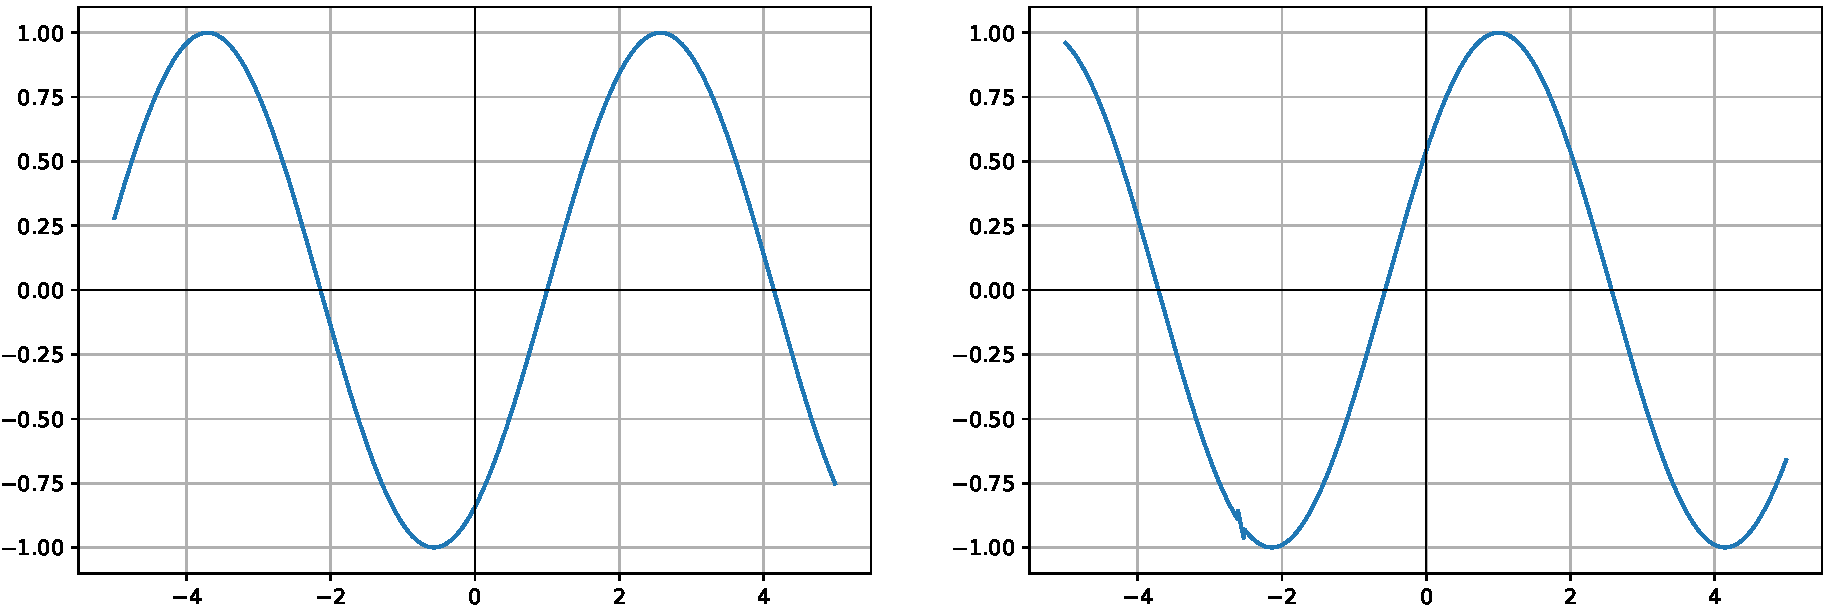
\includegraphics[width=\linewidth]{dpav4_gp_f1.pdf}
  \end{subfigure}
  \begin{subfigure}{\linewidth}
    \centering
    \vspace{2mm}
	\tiny $\cos (x) \cdot 0.9910098031767487$    
    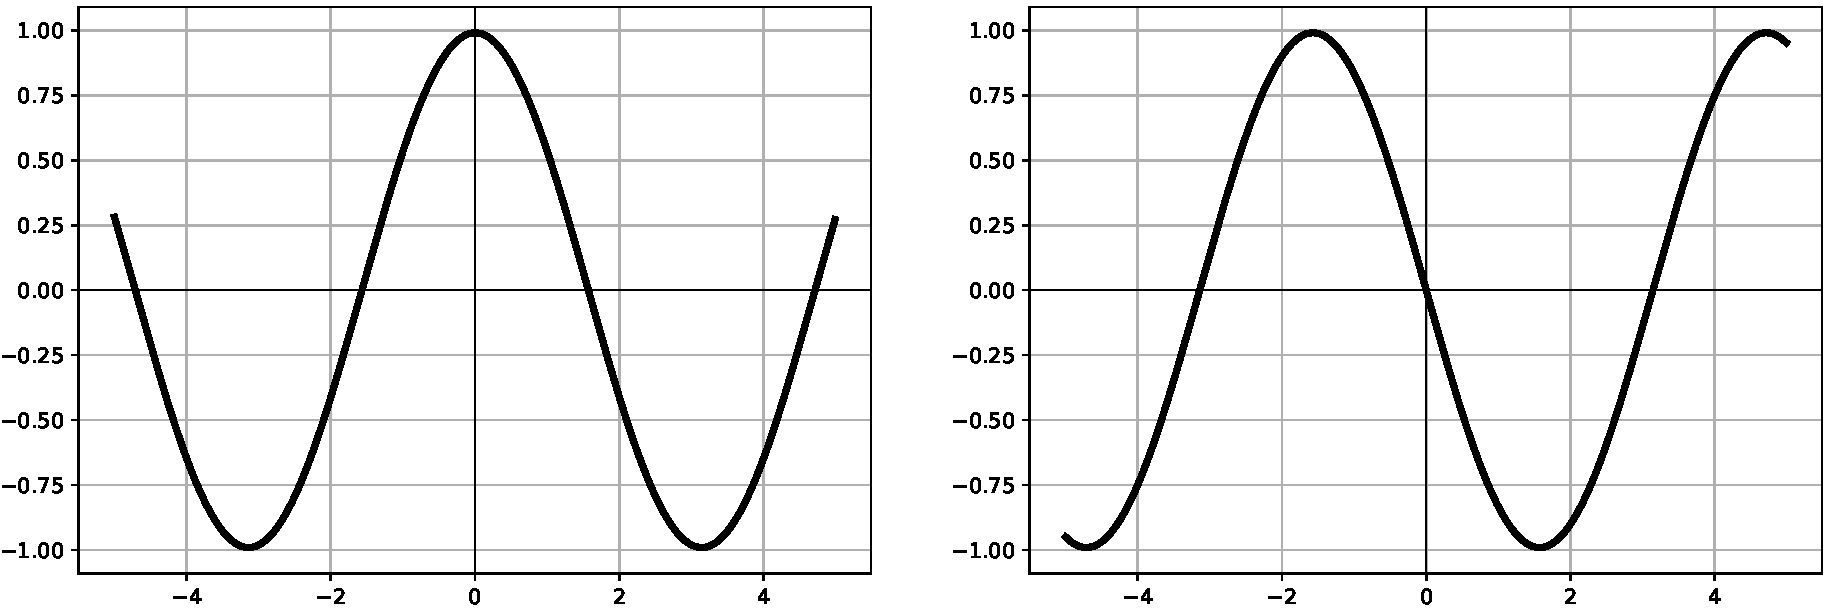
\includegraphics[width=\linewidth]{dpav4_gp_f2.pdf}
  \end{subfigure}
  \begin{subfigure}{\linewidth}
    \centering
    \vspace{2mm}
    \tiny $ReLU (abs (x) \cdot x)$
    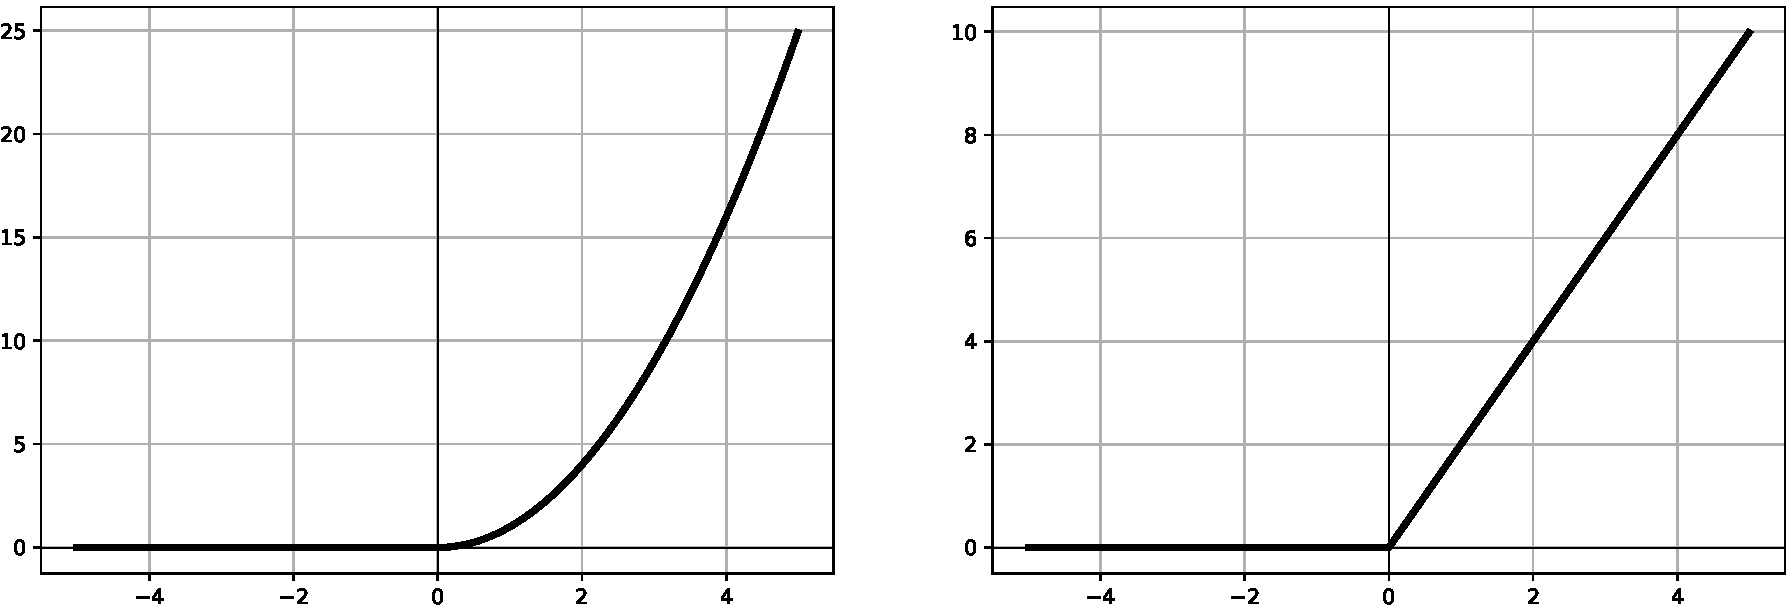
\includegraphics[width=\linewidth]{dpav4_gp_f3.pdf}
  \end{subfigure}
\end{subfigure}
\end{figure}

\end{frame}

%------------------------------------------------
\section{Zaključak}
%------------------------------------------------

\begin{frame}
\frametitle{Zaključak}

\begin{itemize}
\item Odabir AF ima utjecaj na performanse mreže
\item Utjecaj AF može biti nepredvidiv
\item Tabu lista pokazuje znakove poboljšanja
\end{itemize}

Otvorena pitanja za budući rad:

\begin{itemize}
\item Zašto su pronađene AF dobre (distribucija ulaza, kvaliteta gradijenta)?
\item Kakav utjecaj ima periodičnost AF?
\item Kakve AF algoritam pronalazi za dublje arhitekture?
\item Kakav je utjecaj tabu liste na širem skupu evolucijskih algoritmima i problema na kojima se primijenjuju?
\end{itemize}

\end{frame}

\end{document} 
